\documentclass[12pt,a4paper]{extarticle}
\usepackage[utf8]{inputenc}
\usepackage[T5]{fontenc}
\usepackage{geometry}
\geometry{a4paper, left=1.5cm, right=1cm, top=1.5cm, bottom=1.5cm, headheight=20pt, headsep=15pt, footskip=28pt}
\usepackage{enumitem}
\usepackage{amsmath}
\usepackage{amssymb}
\usepackage{diagbox}
\usepackage[most]{tcolorbox}
\newcommand{\khongxacdinh}{\text{KXĐ}}
\newcommand{\blackbox}[1]{\texorpdfstring{\fcolorbox{black}{black}{\textcolor{white}{#1}}}{#1}}
\usepackage{tikz}
\definecolor{bookblue}{RGB}{58,90,172}
\definecolor{book}{RGB}{58,90,172}
\definecolor{myblue}{RGB}{200,40,40}
\newcommand{\bluecheck}{\textcolor{myblue}{\checkmark}}
\newtcolorbox{formulaBox}{colback=gray!5,colframe=bookblue,boxrule=0.8pt,arc=2mm}
\newtcolorbox{notebox}{colback=blue!3,colframe=myblue,boxrule=0.8pt,arc=2mm}
\usetikzlibrary{patterns, patterns.meta} % Thêm patterns.meta vào đây
% Gọi package nằm trong thư mục con template
\usepackage{../template/mngocbox}

\begin{document}

% Sử dụng ngoặc vuông [...] để thay đổi linh hoạt các thông số
\makeheadbox[headerright={Chương 1},chude={Bài 1},tieude={Tính đơn điệu và cực trị của hàm số },dinhdang={Giải tích},lop={12 },gv={Nguyễn Lê Minh Ngọc}]

\vspace{2em}
\makeheading{I}{Kiến thức cần nhớ}


\section*{A. TÍNH ĐƠN ĐIỆU CỦA HÀM SỐ}
\subsection*{I. Định nghĩa}
Kí hiệu $K$ là khoảng hoặc đoạn hoặc nửa khoảng. Giả sử hàm số $y = f(x)$ xác định trên $K$.
\begin{itemize}
	\item Hàm số $y = f(x)$ đồng biến (tăng) trên $K$ nếu với mọi $x_1, x_2$ thuộc $K$ mà $x_1 < x_2$ thì $f(x_1) < f(x_2)$.
	\item Hàm số $y = f(x)$ nghịch biến (giảm) trên $K$ nếu với mọi $x_1, x_2$ thuộc $K$ mà $x_1 < x_2$ thì $f(x_1) > f(x_2)$.
\end{itemize}
Nếu hàm số $y = f(x)$ đồng biến trên $K$ thì đồ thị của nó đi lên từ trái sang phải (hình 1).\\
Nếu hàm số $y = f(x)$ nghịch biến trên $K$ thì đồ thị của nó đi xuống từ trái sang phải (hình 2).
\begin{center}
	\begin{minipage}{0.48\textwidth}
		\centering
		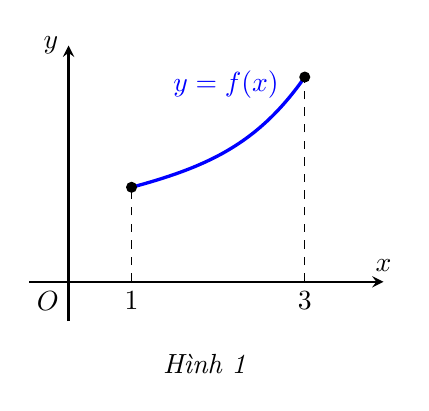
\begin{tikzpicture}[scale=1.0, >=stealth]
			% Axes
			\draw[->, thick] (-0.5,0) -- (4.0,0) node[above] {$x$};
			\draw[->, thick] (0,-0.5) -- (0,3.0) node[left] {$y$};
			\node[below left] at (0,0) {$O$};

			% Curve
			\draw[blue, very thick] (0.8,1.2) to[out=15, in=235] (3.0,2.6);
			\node[above, blue] at (2.0,2.2) {$y = f(x)$};

			% Dashed lines
			\draw[dashed] (0.8,0) node[below] {$1$} -- (0.8,1.2);
			\draw[dashed] (3.0,0) node[below] {$3$} -- (3.0,2.6);

			% Dots
			\fill (0.8,1.2) circle (2pt);
			\fill (3.0,2.6) circle (2pt);

			% Title
			\node[below=0.8cm] at (1.75,0) {\textit{Hình 1}};
		\end{tikzpicture}
	\end{minipage}
	\hfill
	\begin{minipage}{0.48\textwidth}
		\centering
		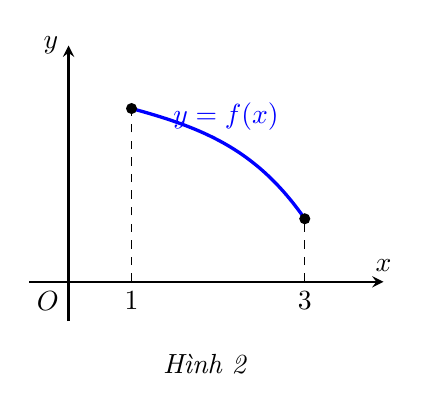
\begin{tikzpicture}[scale=1.0, >=stealth]
			% Axes
			\draw[->, thick] (-0.5,0) -- (4.0,0) node[above] {$x$};
			\draw[->, thick] (0,-0.5) -- (0,3.0) node[left] {$y$};
			\node[below left] at (0,0) {$O$};

			% Curve
			\draw[blue, very thick] (0.8,2.2) to[out=-15, in=125] (3.0,0.8);
			\node[above, blue] at (2.0,1.8) {$y = f(x)$};

			% Dashed lines
			\draw[dashed] (0.8,0) node[below] {$1$} -- (0.8,2.2);
			\draw[dashed] (3.0,0) node[below] {$3$} -- (3.0,0.8);

			% Dots
			\fill (0.8,2.2) circle (2pt);
			\fill (3.0,0.8) circle (2pt);

			% Title
			\node[below=0.8cm] at (1.75,0) {\textit{Hình 2}};
		\end{tikzpicture}
	\end{minipage}
\end{center}
\vspace{0.5cm}
\subsection*{II. Mối quan hệ với đạo hàm}
\begin{tcolorbox}[
		colback=orange!5!white,
		colframe=orange!50!black,
		arc=3mm,
		outer arc=3mm,
		boxrule=1pt,
		enhanced
	]
	Cho hàm số $y = f(x)$ có đạo hàm trên $K$.
	\begin{itemize}
		\item Nếu $f'(x) > 0$ với mọi $x \in K$ thì hàm số $y = f(x)$ đồng biến trên $K$.
		\item Nếu $f'(x) < 0$ với mọi $x \in K$ thì hàm số $y = f(x)$ nghịch biến trên $K$.
	\end{itemize}
\end{tcolorbox}
\vspace{0.5cm}
\noindent $\bullet$ \textbf{Chú ý:} Khi xét tính đơn điệu của hàm số mà chưa cho khoảng $K$, ta hiểu xét tính đơn điệu của hàm số đó trên tập xác định của nó.
\noindent \textbf{Các bước xét tính đơn điệu của hàm số $y = f(x)$:}
\begin{itemize}
	\item \textit{Bước 1.} Tìm tập xác định $D$ của hàm số.
	\item \textit{Bước 2.} Tính đạo hàm $f'(x)$ của hàm số. Tìm các điểm $x_1; x_2; \dots; x_n$ thuộc $D$ mà tại đó đạo hàm $f'(x)$ bằng $0$ hoặc không tồn tại đạo hàm.
	\item \textit{Bước 3.} Sắp xếp các điểm $x_1; x_2; \dots; x_n$ theo thứ tự tăng dần, xét dấu $f'(x)$ và lập bảng biến thiên.
	\item \textit{Bước 4.} Nêu kết luận về các khoảng đồng biến, nghịch biến của hàm số.
\end{itemize}



\section*{B. CỰC TRỊ CỦA HÀM SỐ}

\begin{center}
	\begin{tikzpicture}[scale=1.0, >=stealth]
		% Axes
		\draw[->, thick] (-3.5,0) -- (5.5,0) node[below] {$x$};
		\draw[->, thick] (0,-2.5) -- (0,3.0) node[left] {$y$};
		\node[below left, black] at (0,0) {$O$};

		% Extrema Curve
		\draw[blue, very thick] (-2.8, 1.8)
		.. controls (-2.2, -1.7) and (-2.0, -1.8) .. (-1.8, -1.8)
		.. controls (-1.0, -1.8) and (-0.2, 1.0) .. (0.8, 1.0)
		.. controls (1.5, 1.0) and (2.2, -2.4) .. (3.2, -2.2)
		.. controls (3.8, -2.1) and (4.2, 1.0) .. (4.8, 1.8);

		% Dashed lines to extrema
		\draw[dashed, thick] (-1.8, 0) -- (-1.8, -1.8);
		\draw[dashed, thick] (0.8, 0) -- (0.8, 1.0);
		\draw[dashed, thick] (3.2, 0) -- (3.2, -2.2);

		% Extrema text labels
		\node[below, font=\small] at (-1.8, -1.8) {Điểm cực tiểu};
		\node[above, font=\small] at (0.8, 1.0) {Điểm cực đại};
		\node[below, font=\small] at (3.2, -2.2) {Điểm cực tiểu};

		% Blue arrows for Increasing/Decreasing parts
		\draw[->, red, very thick] (-2.5, 1.0) -- (-2.2, 0.2) node[midway, left, black, font=\small] {Giảm};
		\draw[->, red, very thick] (-1.0, -1.0) -- (-0.4, 0.0) node[midway, right, black, font=\small] {Tăng};
		\draw[->, red, very thick] (1.6, 0.4) -- (2.2, -0.8) node[midway, right, black, font=\small] {Giảm};
		\draw[->, red, very thick] (3.8, -1.4) -- (4.4, -0.2) node[midway, right, black, font=\small] {Tăng};

		% Dots at extrema
		\fill[black] (-1.8, -1.8) circle (2pt);
		\fill[black] (0.8, 1.0) circle (2pt);
		\fill[black] (3.2, -2.2) circle (2pt);
	\end{tikzpicture}
\end{center}

\subsection*{I. Định nghĩa}

Cho hàm số $y = f(x)$ xác định và liên tục trên khoảng $(a; b)$ ($a$ có thể là $-\infty$, $b$ có thể là $+\infty$) và điểm $x_0 \in (a; b)$.
\begin{itemize}
	\item Nếu tồn tại số $h > 0$ sao cho $f(x) < f(x_0)$ với mọi $x \in (x_0 - h; x_0 + h) \subset (a; b)$ và $x \neq x_0$ thì ta nói hàm số $f(x)$ đạt cực đại tại $x_0$.
	\item Nếu tồn tại số $h > 0$ sao cho $f(x) > f(x_0)$ với mọi $x \in (x_0 - h; x_0 + h) \subset (a; b)$ và $x \neq x_0$ thì ta nói hàm số $f(x)$ đạt cực tiểu tại $x_0$.
\end{itemize}

\noindent $\bullet$ \textbf{Chú ý:} Nếu $x_0$ là một điểm cực trị của hàm số $y = f(x)$ thì điểm $M(x_0; f(x_0))$ được gọi là điểm cực trị của đồ thị hàm số $y = f(x)$.

\subsection*{II. Định lý}

Giả sử hàm số $y = f(x)$ liên tục trên khoảng $(a; b)$ chứa điểm $x_0$ và có đạo hàm trên các khoảng $(a; x_0)$ và $(x_0; b)$. Khi đó:
\begin{itemize}
	\item Nếu $f'(x) < 0$ với mọi $x \in (a; x_0)$ và $f'(x) > 0$ với mọi $x \in (x_0; b)$ thì $x_0$ là một điểm cực tiểu của hàm số $f(x)$.
	\item Nếu $f'(x) > 0$ với mọi $x \in (a; x_0)$ và $f'(x) < 0$ với mọi $x \in (x_0; b)$ thì $x_0$ là một điểm cực đại của hàm số $y = f(x)$.
\end{itemize}

\begin{center}
	% Bảng biến thiên cực tiểu
	\begin{minipage}{0.48\textwidth}
		\centering
		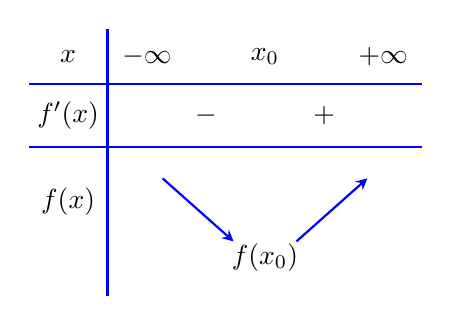
\begin{tikzpicture}[scale=1.0, >=stealth]
			% Các đường kẻ ngang và dọc
			\draw[thick, blue] (0, 1.5) -- (5.0, 1.5);
			\draw[thick, blue] (0, 0.7) -- (5.0, 0.7);
			\draw[thick, blue] (1.0, 2.2) -- (1.0, -1.2);

			% Các nhãn ở cột đầu tiên
			\node at (0.5, 1.85) {$x$};
			\node at (0.5, 1.1) {$f'(x)$};
			\node at (0.5, 0.0) {$f(x)$};

			% Hàng giá trị x
			\node at (1.5, 1.85) {$-\infty$};
			\node at (3.0, 1.85) {$x_0$};
			\node at (4.5, 1.85) {$+\infty$};

			% Hàng dấu f'(x)
			\node at (2.25, 1.1) {$-$};
			\node at (3.75, 1.1) {$+$};

			% Chiều biến thiên f(x) với mũi tên đi xuống rồi đi lên
			\node (mid1) at (3.0, -0.7) {$f(x_0)$};
			\draw[->, blue, thick] (1.7, 0.3) -- (2.6, -0.5);
			\draw[->, blue, thick] (3.4, -0.5) -- (4.3, 0.3);
		\end{tikzpicture}
	\end{minipage}
	\hfill
	% Bảng biến thiên cực đại
	\begin{minipage}{0.48\textwidth}
		\centering
		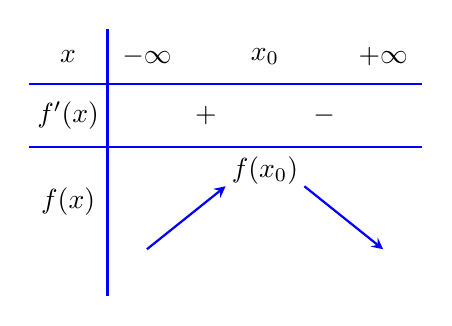
\begin{tikzpicture}[scale=1.0, >=stealth]
			% Các đường kẻ ngang và dọc
			\draw[thick, blue] (0, 1.5) -- (5.0, 1.5);
			\draw[thick, blue] (0, 0.7) -- (5.0, 0.7);
			\draw[thick, blue] (1.0, 2.2) -- (1.0, -1.2);

			% Các nhãn ở cột đầu tiên
			\node at (0.5, 1.85) {$x$};
			\node at (0.5, 1.1) {$f'(x)$};
			\node at (0.5, 0.0) {$f(x)$};

			% Hàng giá trị x
			\node at (1.5, 1.85) {$-\infty$};
			\node at (3.0, 1.85) {$x_0$};
			\node at (4.5, 1.85) {$+\infty$};

			% Hàng dấu f'(x)
			\node at (2.25, 1.1) {$+$};
			\node at (3.75, 1.1) {$-$};

			% Chiều biến thiên f(x) với mũi tên đi lên rồi đi xuống
			\node (mid2) at (3.0, 0.4) {$f(x_0)$};
			\draw[->, blue, thick] (1.5, -0.6) -- (2.5, 0.2);
			\draw[->, blue, thick] (3.5, 0.2) -- (4.5, -0.6);
		\end{tikzpicture}
	\end{minipage}
\end{center}



\end{document}